\section{Oppenheimer-Snyder collapse and strong scaling}\label{sec:collapse}

Full three-plus-one numerical relativity coupling tests dynamic spacetime deposition, adaptive mesh refinement, lapse excision, and apparent horizon tracking in Oppenheimer-Snyder spherical dust collapse \cite{Oppenheimer:1939ue}. Following standard self-gravitating initial data \cite{Wu:2026nrpic}, we initialize a cold ($u_i = 0$, $\Sigma = 0$), initially static homogeneous dust sphere of isotropic radius $\bar{R}_0 \approx 4.48M$ (areal radius $R_0 = 5M$, unit rest mass) on a seven-level adaptive grid covering $[-155M, 155M]^3$ with L{\"o}hner metric refinement, Z4c evolution under Bona-Masso $1+\log$ slicing \cite{Bona:1994dr,Bona:2003fj} and Gamma-driver shift \cite{Alcubierre:2002kk,Campanelli:2005dd}, one binomial deposit filter pass, and lapse excision below $\alpha_{\rm exc} = 0.1$. A zero-temperature basis automatically collapses the fifth-degree cubature rule in Eq.~(\ref{eq:scp_map}) to $Q_{\rm SCP} = 1$ packet per populated element, yielding $N = 9328$ cold packets deposited onto the Z4c right-hand side.

\begin{figure}[t]
\centering
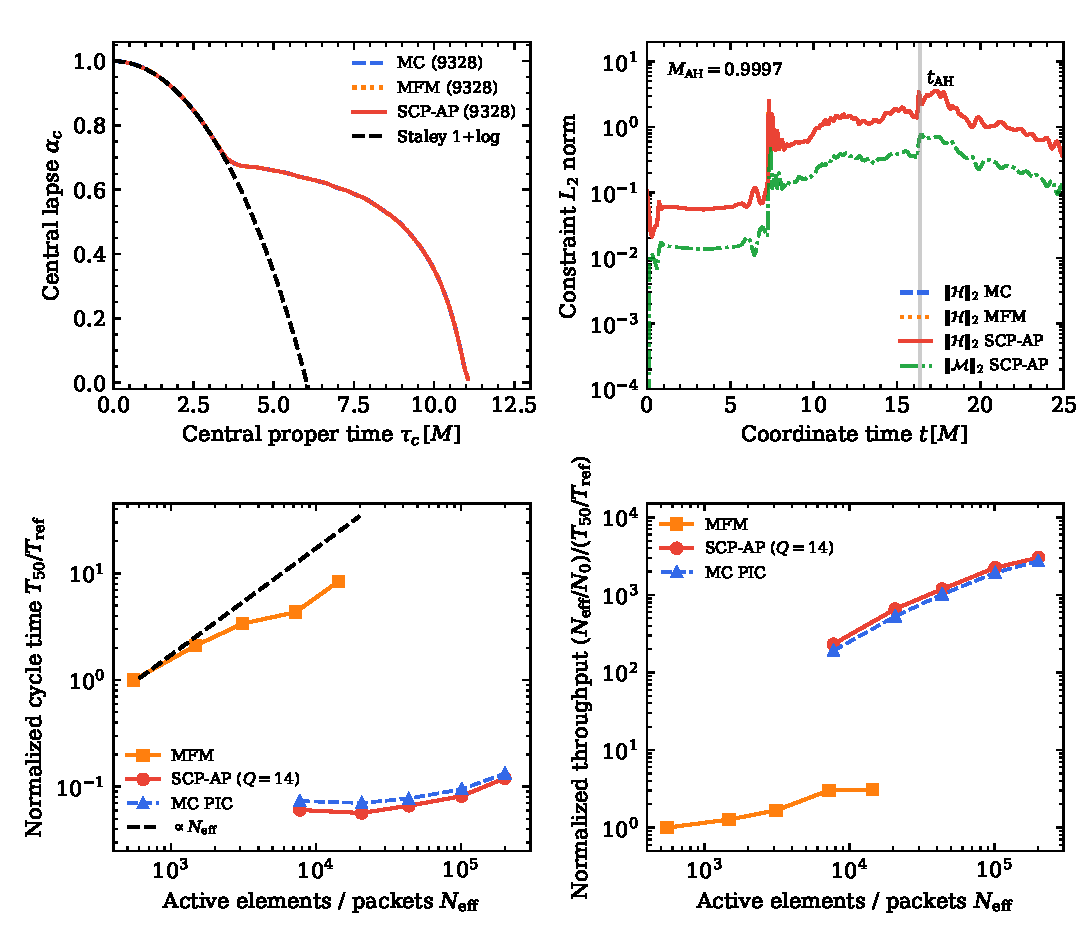
\includegraphics[width=\columnwidth]{figures/fig_os_and_scaling.pdf}
\caption{\label{fig:os_and_scaling}%
Dynamical collapse and strong scaling. Top left: Central lapse $\alpha_c(\tau_c)$ during $R_0 = 5M$ collapse vs Staley bound. Top right: Z4c norms $\|\mathcal{H}\|_2$ and $\|\mathcal{M}\|_2$, horizon time $t_{\rm AH}$, and mass $M_{\rm AH} = 0.9997M$. Bottom left: Normalized $50$-cycle compute time vs $N_{\rm eff}$. Bottom right: Normalized throughput.}
\end{figure}

As collapse proceeds through $t = 25M$, all three kinetic discretizations (Monte Carlo PIC, continuum MFM, and cold SCP-AP packets) produce virtually indistinguishable spacetime and matter histories. In Fig.~\ref{fig:os_and_scaling} (top-left panel), the central lapse $\alpha_c(\tau_c)$ tracks the analytical Staley lower bound $\alpha_{\rm LL} = 1 + 6 \ln(R/R_0)$ \cite{Staley:2011ss} closely in early collapse before trumpet slicing slows proper time near $\alpha_c \to 0$ at $\tau_c \approx 11.1M$. FastFlow \cite{Gundlach:1997us} detects the apparent horizon identically at $t_{\rm AH} = 16.39M$ with final irreducible mass $M_{\rm AH} \approx 1.00M$ across all three methods, while $99$ percent rest-mass lapse excision completes at $t_{\rm exc} = 19.71M$. Global Z4c Hamiltonian and momentum constraint $L_2$ norms ($\|\mathcal{H}\|_2$ and $\|\mathcal{M}\|_2$, top-right panel) overlap closely across refinement transitions around $t \approx 7M$ and horizon formation. The overlapping trajectories demonstrate dynamical Einstein-Vlasov compatibility without stability loss or excision drift.

Strong scaling in curved Kerr geometry quantifies algorithmic throughput as phase-space resolution rises across nearly three decades from $N_{\rm eff} = 552$ up to $N_{\rm eff} = 200592$ packets over fifty fixed RK2 cycles (bottom panels of Fig.~\ref{fig:os_and_scaling}, normalized to baseline $N_0 = 552$ continuum MFM compute time $T_{\rm ref}$). Continuum MFM compute cost grows roughly linearly beyond $N \sim 3 \times 10^3$ elements once neighbor-stencil assembly and pairwise face fluxes saturate device memory bandwidth, reaching $T_{50} / T_{\rm ref} \approx 8.4$ at $N = 14328$. By bypassing spatial neighbor graphs, gradient limiters, and pairwise Riemann solves, the SCP-AP branch sustains nearly flat sub-linear runtime up to $N_{\rm eff} \approx 4 \times 10^4$ packets before transitioning cleanly to high-throughput parallel streaming at $T_{50} / T_{\rm ref} \approx 0.12$ for $200592$ packets. At matched lattice resolution ($N_{\rm lat} = 30$, $14328$ elements expanded to $200592$ packets), normalized update throughput of SCP-AP exceeds continuum MFM by roughly three orders of magnitude per tracer and achieves nearly seventyfold lower absolute compute time per cycle while closely matching pure Monte Carlo particle pushers.
